\chapter{Theory}\label{cha:theory}

\begin{comment}
The background theory depth and breadth depend on the depth needed to understand your project
in the different disciplines that your project crosses.
It is not a place to just write about everything you know that is vaguely connected to your project.
The theory is here to help the readers that do not know the theoretical basis of your work so that they
can gain sufficient understanding to understand your contributions --- and also for yourself to show that
you have understood the underlying theory and are aware of the methods used in the field.
In particular, the theory section provides
an opportunity to introduce terminology that can later be used without disturbing the text with a definition.
In some cases it will be more appropriate to have a separate section for different theories (or even separate chapters).
However, be careful so that you do not end up with too short sections.
Subsections may also be used to separate different background theories.

Be aware that ``background'' is a general term that refers to everything done by somebody else,
in contrast to the ``foreground'', which is your own work.
Hence there can (and will) be several background chapters, with the background theory being one of them
--- or several of them, since it thus is quite possible to split the background theory over more than one chapter,
e.g., by having a chapter introducing the theory directly needed for the research field in question and another
chapter discussing the machine learning theory, algorithms, tools, and evaluation methods commonly used in the field.
The related work chapter is thus also part of the background, while a chapter about data might be background
(if you only use somebody else datasets), but can also be part of the foreground (if you collect and/or annotate data
yourself, or if you process or clean the data in ways that can make it part of your own contribution).

It is ok to reuse material from other texts that you have written (e.g., the specialisation project), but if you do so, that must be clearly stated in the text, together with a description of how much of the text is new, old or rewritten/edited.
Such a statement about recycling of material in the Background Theory chapter can thus come here in the chapter introduction.

\section{Writing References in the Text}
\label{sec:writing_references}

When introducing techniques or results, always reference the source.
Be careful to reference the original contributor of a technique and not just someone who happens to use the technique.%
\footnote{But always make sure that you have read the work you are citing --- if not, cite someone who has!}
For results relevant to your work,
you would want to look particularly at newer results so that you have referenced the most up-to-date work in your area.
A common rule of thumb is to at least reference the first paper introducing the issue and the paper containing the latest / state-of-the-art
results. Additional papers making substantial contributions should also be referenced, as well as of course the ones you find most interesting.
Remember to use the right verb form depending on the number of authors.

If you do not have the source handy when writing, mark in the text that a reference is needed and add it later. \todo{add reference}
Web pages are not reliable sources --- they might be there one day and removed the next; and thus should be avoided, if possible.
A verbal discussion is not a source and should normally not be referenced
(though you can reference ``personal communication'', if there are no other options).
The bulk of citations in the report will appear in Chapter~\ref{cha:related_work}.
However, you will often need to introduce some terminology and key citations already in this chapter.

You can cite a paper in the following manner (and several other versions,
see the \verb!natbib! package documentation):

\section{The Reference List}
\label{sec:reference_list}

In general, make sure that the references that appear in your reference list can be easily located and identified by the reader.
So include not only authors and title, but year and place of publication, the full names of conferences and workshops,
page numbers in proceedings and collections, etc.
Hyperlinks or \acrfull{acr:doi} numbers are also nice to include.
Just as in the text itself, it is important to be consistent in the reference list, so include the same type of information for all references and write it in the same way.

% Check out the reference list at the end of this document for examples of how to write references in \BibTeX.
% Note a particular quirk: Many \BibTeX\ styles convert uppercase letters to lowercase, unless specifically told not to.
% You might thus need to ``protect'' characters that should not be converted, e.g., by writing \texttt{\{T\}witter} as in the \citet{FountaEA:18} reference.

% Also, keep in mind that `et' is a word in its own right (`and'), so there is no period after it (even though there is a period after `al.', which is short for `alia', meaning `others').
% Of course, when including such a reference in the text, the authors should be referred to in plural form. 
% So \citet{BenyonEA:13} state that life is good (not ``states'').

% Many sites, such as journals and \url{dblp.org} provide the matching \BibTeX\ entry for a reference. 
% However, you might still need to edit the entry in order to be consistent with the rest of your references.
% If you find references from sites such as \url{scholar.google.com} or \url{arXiv.org}, keep in mind that they often not are complete,
% so that you might need to add information to the entry (and probably edit it as well).

Some other good sites to find state-of-the-art work:
\begin{itemize}
    \item \url{paperswithcode.com}
    \item \url{nlpprogress.com}

\end{itemize}

\textit{Lorem ipsum dolor sit amet, consectetur adipiscing elit, sed do eiusmod tempor incididunt ut labore et dolore magna aliqua. Ut enim ad minim veniam, quis nostrud exercitation ullamco laboris nisi ut aliquip ex ea commodo consequat. Duis aute irure dolor in reprehenderit in voluptate velit esse cillum dolore eu fugiat nulla pariatur. Excepteur sint occaecat cupidatat non proident, sunt in culpa qui officia deserunt mollit anim id est laborum.}


\section{Introducing Figures}

\LaTeX is a bit tricky when it comes to the placement of ``flooting bodies'' such as figures and tables. It is often a good idea to let their code appear right before the header of the (sub)section in which they appear.
Note that you should anyhow always use an option for the placement (e.g., \verb|[t!]| to place it at the top of a page).

Do not just put the figure in and leave it to the reader to try to understand what the figure is.
The figure should be included to convey a message and you need to help the reader to understand the message
intended by explaining the figure in the text.
Hence \textbf{all} figures and tables should always be referenced in the text, using the \verb!\ref! command.
It is good practice to always combine it with a non-breakable space (\verb!~!) so that there will be no newline between the term referring to it and the reference, that is, using \verb!Figure~\ref{fig:BoxesAndArrowsAreNice}!.

Also, note that you can have a longer version of the figure (and table) caption attached to the actual figure,
while using the optional first argument to \verb!\caption! to include a shorter version in the list of figures (lof) or list of tables:
\begin{quote}
    \begin{verbatim}
\caption[Shorter lof text]{Longer text appearing under the figure}
\end{verbatim}
\end{quote}

\begin{figure}[t!]
    \centering
    \missingfigure{Here we will add an amazing figure explaining it all}
    \caption{A missing figure}
    \label{fig:AmazingFigure}
\end{figure}

In general it is good to add notes about things that you plan on writing later.
The \verb!todonotes! package is great for that kind of book-keeping, letting you write both shorter comments in the margin\todo{l8r dude} and longer comments inside the text, using the option \verb![inline]!.
\todo[inline]{There are always some more stuff that you will need to add at some later point.
    Be sure to at least make a note about it somewhere.}

\textit{Sed ut perspiciatis unde omnis iste natus error sit voluptatem accusantium doloremque laudantium, totam rem aperiam, eaque ipsa quae ab illo inventore veritatis et quasi architecto beatae vitae dicta sunt explicabo. Nemo enim ipsam voluptatem quia voluptas sit aspernatur aut odit aut fugit, sed quia consequuntur magni dolores eos qui ratione voluptatem sequi nesciunt. Neque porro quisquam est, qui dolorem ipsum quia dolor sit amet, consectetur, adipisci velit, sed quia non numquam eius modi tempora incidunt ut.}

\section{Introducing Tables in the Report}

\newcommand\emc{-~~~~}
\begin{table}[t!]
    \centering
    \caption[Example table]{Example table (F$_1$-scores); this table uses the optional shorter caption that will appear in the list of tables, so this long explanatory text will not appear in the list of tables and is only here in order to explain that to the reader.}
    \begin{tabular}{c|c|rrrrrr}
        \tabletop
        Langs                  & Source                                           & \multicolumn{1}{c}{Lang1} & \multicolumn{1}{c}{Lang2} & \multicolumn{1}{c}{Univ} & \multicolumn{1}{c}{NE} & \multicolumn{1}{c}{Mixed} & \multicolumn{1}{c}{Undef}
        \\ \tablemid
        \multirow{5}{*}{EN-HI} & FB+TW                                            & 54.22                     & 22.00                     & 19.70                    & 4.00                   & 0.05                      & 0.03                      \\
                               & FB                                               & 75.61                     & 4.17                      & 18.00                    & 2.19                   & 0.02                      & 0.01                      \\
                               & TW                                               & 22.24                     & 48.48                     & 22.42                    & 6.71                   & 0.08                      & 0.07                      \\
                               & Vyas                                             & 54.67                     & 45.27                     & 0.06                     & \emc                   & \emc                      & \emc                      \\
                               & FIRE                                             & 45.57                     & 39.87                     & 14.52                    & \emc                   & 0.04                      & \emc                      \\ \tablemid
        \multirow{2}{*}{EN-BN} & TW                                               & 55.00                     & 23.60                     & 19.04                    & 2.36                   & \emc                      & \emc                      \\
                               & FIRE                                             & 32.47                     & 67.53                     & \emc                     & \emc                   & \emc                      & \emc                      \\ \tablemid
        EN-GU                  & FIRE                                             & 5.01                      & \textbf{94.99}            & \emc                     & \emc                   & \emc                      & \emc                      \\
        \tablemid
        DU-TR                  & Nguyen                                           & 41.50                     & 36.98                     & 21.52                    & \emc                   & \emc                      & \emc                      \\ \tablemid

        EN-ES                  & \multirow{4}{*}{\rotatebox[origin=c]{90}{EMNLP}}
                               & 54.79                                            & 23.50                     & 19.35                     & 2.08                     & 0.04                   & 0.24                                                  \\
        EN-ZH                  &                                                  & 69.50                     & 13.95                     & 5.88                     & 10.60                  & 0.07                      & \emc                      \\
        EN-NE                  &                                                  & 31.14                     & 41.56                     & 24.41                    & 2.73                   & 0.08                      & 0.08                      \\
        AR-AR                  &                                                  & 66.32                     & 13.65                     & 7.29                     & 11.83                  & 0.01                      & 0.90                      \\ \tablebot
    \end{tabular}
    \label{tab:ExampleTable}
\end{table}

As you can see from Table~\ref{tab:ExampleTable}, tables are nice.
However, again, you need to discuss the contents of the table in the text.
You do not need to describe every entry, but draw the reader's attention to what is important in the table,
e.g., that 94.99 is an amazing F$_1$-score (and that probably something fishy happened there).
Use boldface, boxes, colours, arrows, etc. to mark the important parts of the table.

As can be seen in the example, elements in a table can sometimes benefit from being rotated (such as EMNLP in the `Source' column) or cover more than one row (EMNLP, as well as EN-HI and EN-BN in the `Langs' column) --- or more than one column, for that matter.
\end{comment}

\textit{Disclaimer: I will reuse parts of a paper I wrote in the theory module called "TDT13 - Advanced Text Analytics and Language Understanding" in this \autoref{cha:theory} chapter. This includes \autoref{subsec:attention-and-transformers} and \autoref{subsec:bert}.}

\vspace{12pt}

\Autochapterref{cha:theory} of this specialization project will talk about the leading technologies in the field of \gls{acr:llm}, which in itself is a subfield of \gls{acr:nlp}. \autoref{sec:llms} will go over the leading \gls{acr:llm} models, their strengths and weaknesses, and briefly mention differences in model architecture. \Autosectionref{sec:llm-providers} will name the most prominent providers of \gls{acr:llm} services.

\autoref{fig:actor-map} shows an actor map which includes stakeholders, providers, and other groups and organizations that could have some relevance to an autonomous LLM-based GIS-agent. Following subsections will go over the different groups and explain why they are included in the actor map.

\begin{figure}
    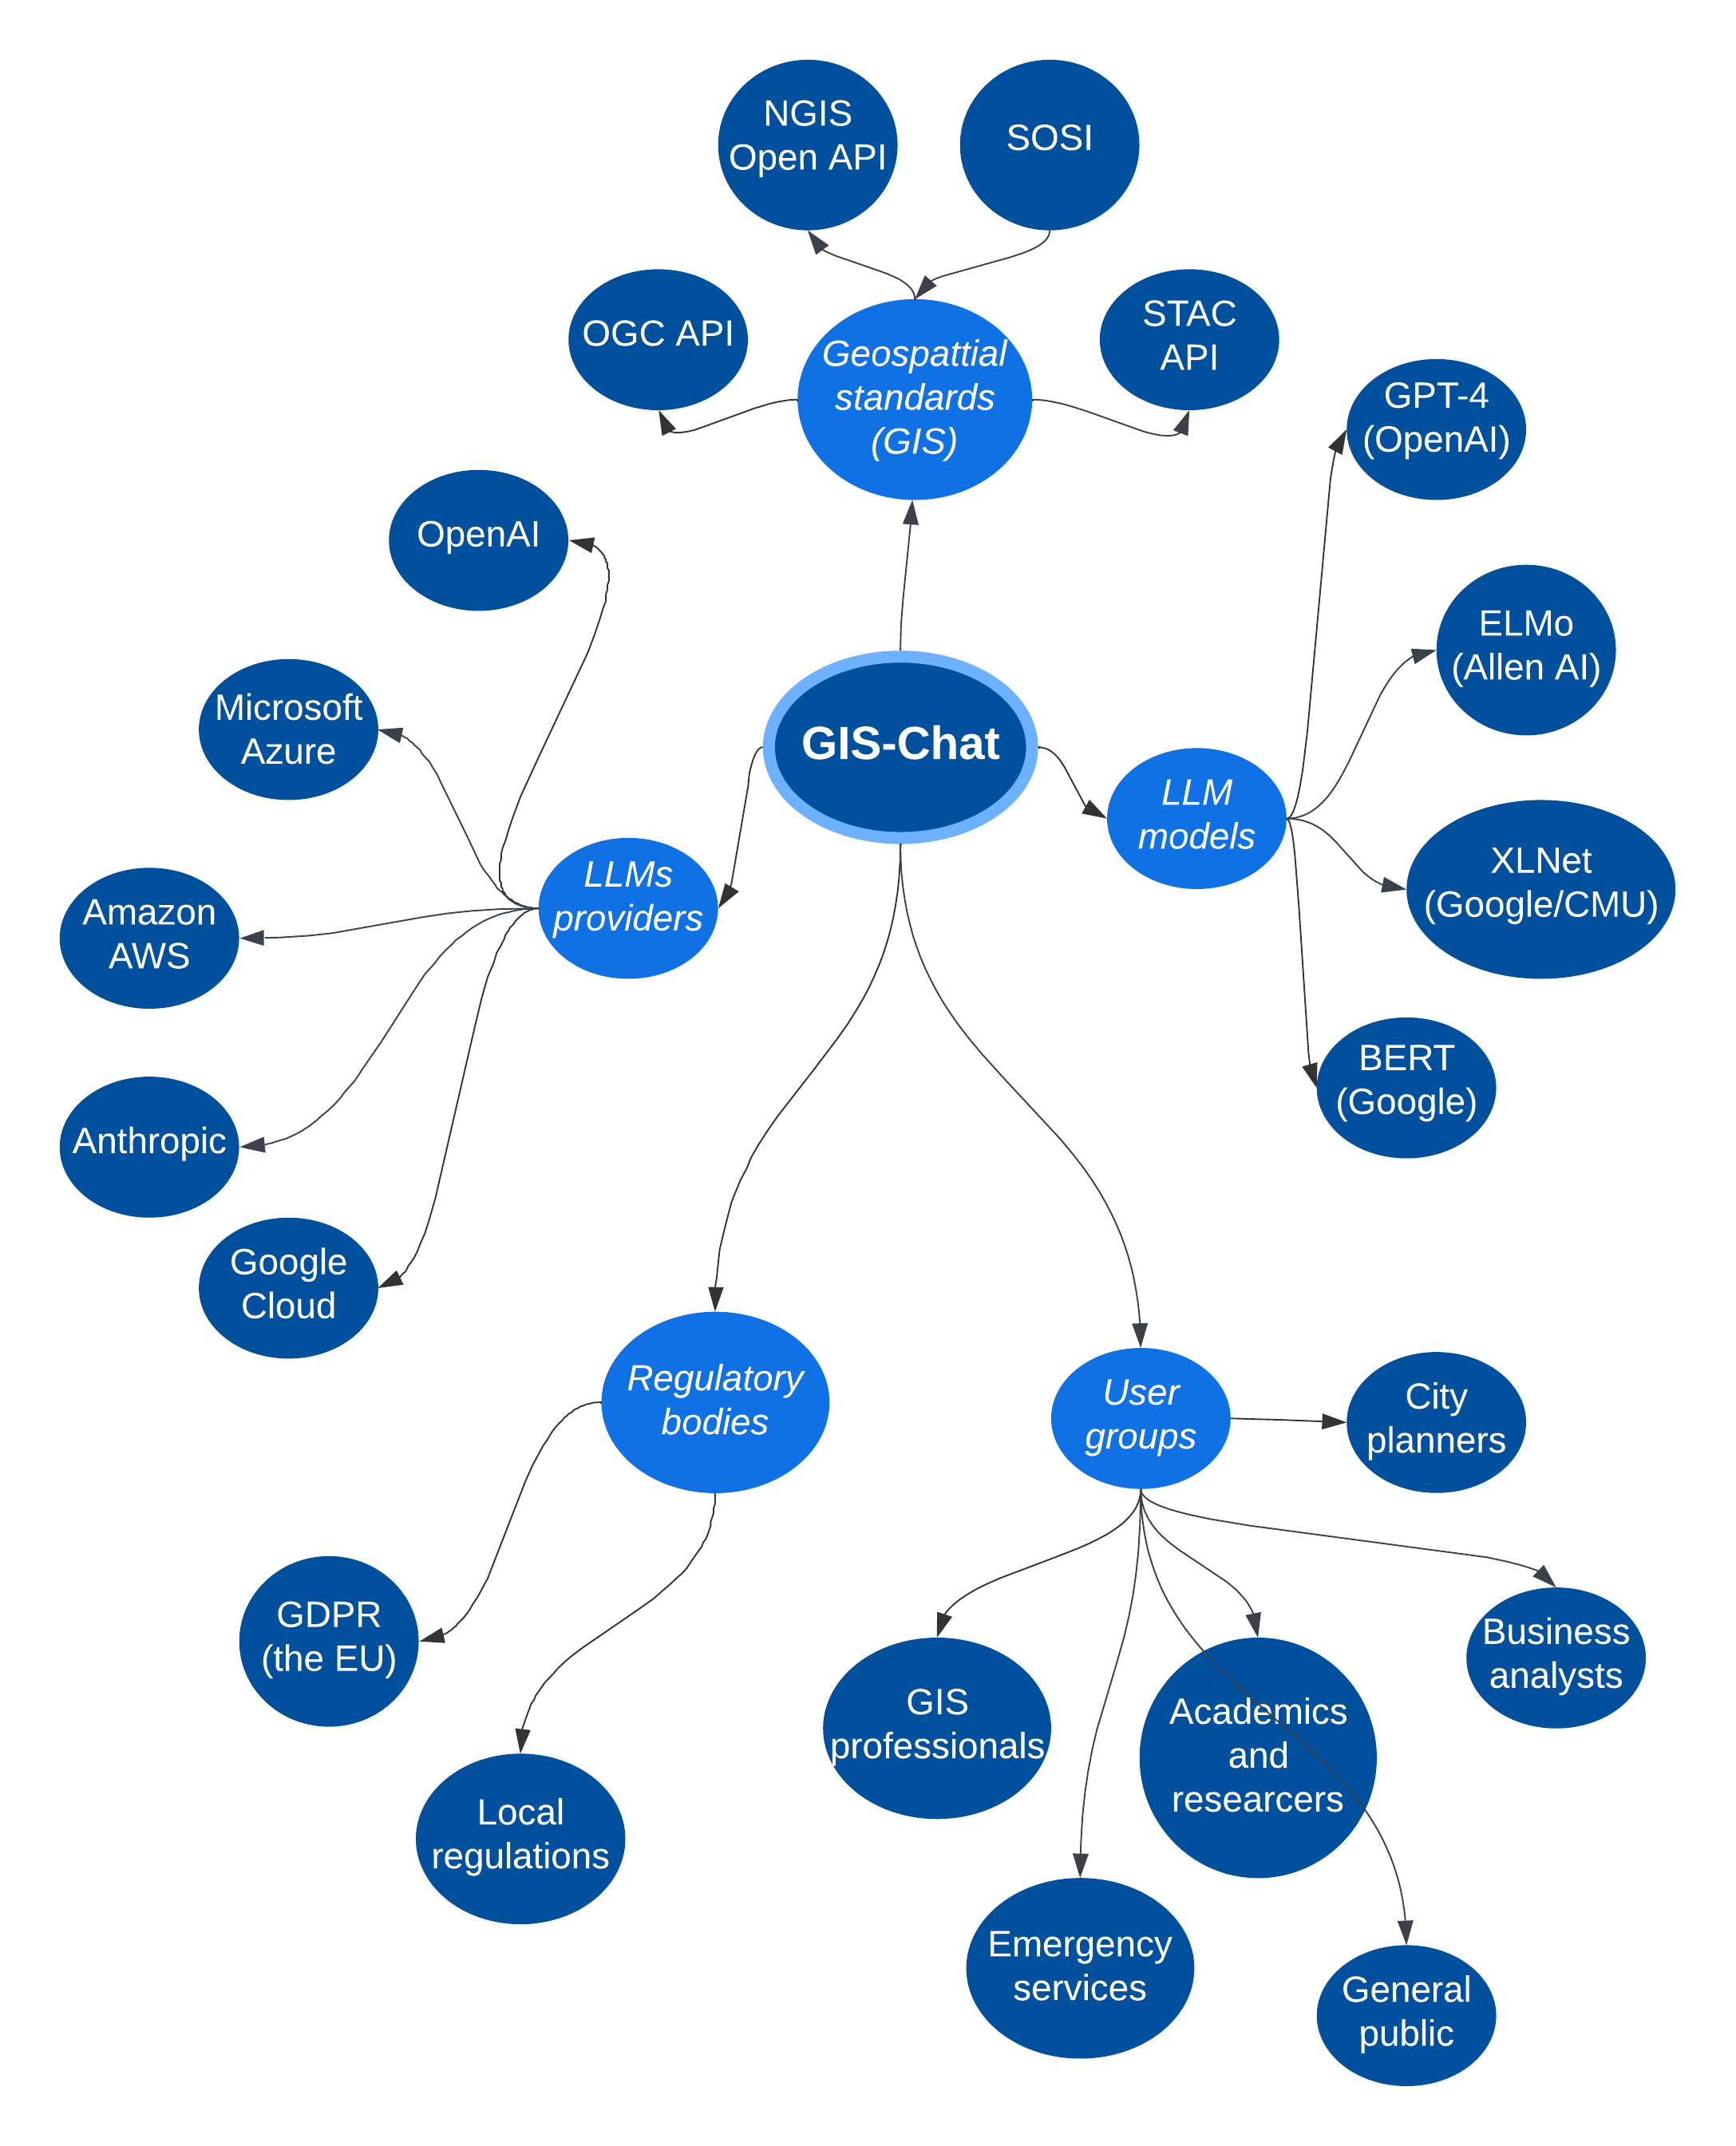
\includegraphics[width=\textwidth]{actor_map}
    \caption{Actor map for stakeholders, providers, and other groups and organizations that could have some relevance to an autonomous LLM-based GIS-agent.}
    \label{fig:actor-map}
\end{figure}

\section[Large Language Models]{\acrshortpl{acr:llm}}\label{sec:llms}

This section will open with an explanation of the building block of modern \acrlongpl{acr:llm}, namely the Transformer, which employs self-attention. \Autosubsectionref{subsec:gpt} and \autoref{subsec:bert} will then discuss the two most famous families of \acrshortpl{acr:llm}, namely the \acrshort{acr:gpt}'s and the \acrshort{acr:bert}'s, as well as the brand new multimodal Gemini model from Google, and various open-source alternatives. \Autosectionref{sec:benchmarking-and-evaluation} will then enlighten the reader about the different ways in which \acrlongpl{acr:llm} can be benchmarked and how we can measure the quality of a natural language response produced by an \acrshort{acr:llm}.

\subsection{Attention and The Transformer Architecture}\label{subsec:attention-and-transformers}

\cite{vaswaniAttentionAllYou2017} managed to achieve new state-of-the-art results for machine translation tasks with their introduction of the Transformer architecture. The Transformer has later been proved effective for numerous downstream tasks, and for a variety of modalities. Titling their paper \citetitle{vaswaniAttentionAllYou2017}, \citeauthor{vaswaniAttentionAllYou2017} suggest that their attention-based architecture renders \glspl{acr:rnn} redundant, due to its superior parallelization abilities and the shorter path between combinations of position input and output sequences, making it easier to learn long-range dependencies \citep[6]{vaswaniAttentionAllYou2017}.

The Transformer employs self-attention, which enables the model to draw connections between arbitrary parts of a given sequence, bypassing the long-range dependency issue commonly found with \glspl{acr:rnn}. An attention function maps a query and a set of key-value pairs to an output, calculating the compatibility between a query and a corresponding key \citep[3]{vaswaniAttentionAllYou2017}. Looking at \citeauthor{vaswaniAttentionAllYou2017}'s proposed attention function \eqref{eq:attention}, we observe that we take the dot product between the query $Q$ and the keys $K$, where $Q$ is the token that we want to compare all the keys to. Keys similar to $Q$ will get a higher score, e.g., be \textit{more attended to}. These differences in attention are further emphasized by applying the softmax function. The final matrix multiplication with the values $V$, being the initial embeddings of all input tokens, will give us a new embedding in which all tokens have some context from all other words. We improve the attention mechanism by multiplying queries, keys, and values with weight matrices learned through backpropagation. Self-attention is a special kind of attention in which queries, keys, and values are all the sequence.

\begin{equation}
    \text{Attention}(Q, K, V) = \text{softmax}\left(\frac{QK^T}{\sqrt{d_k}}\right)V
    \label{eq:attention}
\end{equation}

Attention blocks can be found in three places in the Transformer architecture \citep[5]{vaswaniAttentionAllYou2017} (I will use machine translation from Norwegian to German as an example):

\begin{enumerate}
    \item In the encoder block to perform self-attention on the input sequence (which is in Norwegian)
    \item In the decoder block to perform self-attention on the output sequence (which is in German)
    \item In the decoder block to perform cross-attention (or encoder-decoder attention) where each position in the decoder attends to all positions in the encoder
\end{enumerate}

The Transformer represented a breakthrough in the field of \gls{acr:nlp}, and is the fundamental building block of \acrshortpl{acr:llm} like \acrshort{acr:bert}.


\subsection[The GPT Family]{The \acrshort{acr:gpt} Family}\label{subsec:gpt}

\glspl{acr:gpt} are a type of \gls{acr:llm} first introduced by \hyperref[subsec:openai]{OpenAI} in 2018 \citep{radfordImprovingLanguageUnderstanding2018}. Specifically designed to perform text generation, it is essentially a stack of Transformer \textit{decoders}, and demonstrates through its vast training on unlabelled data help a language model learn good representations, providing a significant performance boost, while alleviating the dependence on supervised learning. While the original Transformer architecture as described by \cite{vaswaniAttentionAllYou2017} was intended for machine translation, thus having encoder to learn the representation of the origin language representation of a given input sequence and an encoder to learn the representation in the target language and perform cross-attention between the two, the \acrshort{acr:gpt} is designed only to \textit{imitate} language. By applying masked multi-head attention, the model is restricted to only see past $k$ (with $k$ being the size of the context window) tokens and is tasked to predict the next one.

Training consists of two stages: unsupervised pre-training and supervised fine-tuning. The former is used to find a good initialization point, essentially teaching the model to imitate the corpora it is trained upon. This results in a model that will ramble on uncontrollably, just trying to complete the input sequence it's given to the best of its knowledge, however this will produce undefined behaviour. It is therefore necessary to fine-tune the model on a target task with supervision. \cite[4]{radfordImprovingLanguageUnderstanding2018} explain how the model can fine-tune directly on tasks like text classification, but how one for other tasks needs to convert structured inputs into ordered sequences because the pre-trained model was trained on contiguous sequences of text. In the case of ChatGPT, \citeauthor{openaiIntroducingChatGPT2022} used \gls{acr:rlhf} by employing a three-step strategy: first training using a supervised policy, then using trained reward models to rank alternative completions produced by ChatGPT models, before fine-tuning the model using \gls{acr:ppo}. This pipeline is then performed for several iterations until the model produces the desired behaviour \citep{openaiIntroducingChatGPT2022}.

\subsection[The BERT Family]{The \acrshort{acr:bert} Family}\label{subsec:bert}

\gls{acr:bert}, introduced about four months after release of paper on the \acrshort{acr:gpt} architecture \citep{radfordImprovingLanguageUnderstanding2018}, is a family of language models which was first introduced in 2018 and is designed to facilitate a wide range of downstream tasks \citep[5]{devlinBERTPretrainingDeep2019}. The \acrshort{acr:bert} architecture consists of stacked bidirectional Transformer \textit{encoders}. This makes \acrshort{acr:bert} unsuitable for text generation, unlike the \textit{decoder}-based \acrshort{acr:gpt} architecture. However, the self-attention in the encoder, in which tokens can \textit{see} both past and future tokens, mechanism allows for training of deep bidirectional representations, facilitating a wide range of \gls{acr:nlp} tasks. The input sequence is transformed into embeddings (vector representations). These per-token embeddings include information about the meaning of the word itself, the meaning of the sentence/segment it belongs to, and the token's position in the full input. These embeddings then pass through a stack of Transformer encoders (12 and 24 for \textbf{\acrshort{acr:bert}\textsubscript{BASE}} and \textbf{\acrshort{acr:bert}\textsubscript{LARGE}}, respectively), allowing the model to learn more complex patterns and of different granularities (token, sentence, document) \citep[5]{devlinBERTPretrainingDeep2019}.

In the \acrshort{acr:bert} framework, there are two training steps, namely the pre-training and fine-tuning procedures. \acrshort{acr:bert} is pre-trained on two \acrshort{acr:nlp} tasks. One is \gls{acr:mlm}, in which 15\% of words are masked with the special \texttt{[MASK]} token and are left for the model to predict \citep[4]{devlinBERTPretrainingDeep2019}. The \gls{acr:mlm} task helps the model learn bidirectional representations. The second of the two unsupervised tasks used during pre-training is \gls{acr:nsp}, where the special \texttt{[CLS]} token (found at the start of each tokenized sequence) is used to predict if a sentence \texttt{B} follows \texttt{A}. During this pre-training step, the input sequence looks like this:

$$
    \texttt{[CLS]} \text{ this is sentence A } \texttt{[SEP]} \text{ and this is sentence B } \texttt{[SEP]}
$$

The \texttt{[CLS]} token is used to label sentence B as either \texttt{IsNext} or \texttt{NotNext}.

\acrshort{acr:bert} is normally fine-tuned to specific downstream tasks by using the \texttt{[CLS]} token, which captures an aggregated representation of the input sequence. This vector representation can then be used as input to a classification layer for tasks like multi-label classification and regression.

\subsection{Gemini}\label{subsec:gemini}

As of writing, Google's Gemini \citep{geminiteamGeminiFamilyHighly2023} (introduced on December 6th 2023) is the latest addition to the field of \acrshortpl{acr:llm}. Being fundamentally designed for multimodality, it is able to reason between text, images, video, audio, and code. Is released in different sizes: the Gemini Ultra, the Gemini Pro, and the Gemini Nano. The Gemini Ultra produces state-of-the-art performance on 30 of 32 widely-used academic benchmarks, and performs worse than \citeauthor{openaiGPT4TechnicalReport2023}'s \acrshort{acr:gpt}-4 on only one benchmark, the HellaSwag benchmark for common-sense reasoning for everyday tasks. Gemini Ultra outperforms \acrshort{acr:gpt}-4 on the \acrshort{acr:mmlu} benchmark, various reasoning benchmarks, and shows significant improvements in maths and code related benchmarks  \citep[7]{geminiteamGeminiFamilyHighly2023}. Gemini performs better than \citeauthor{openaiGPT4TechnicalReport2023}'s multimodal equivalent of \acrshort{acr:gpt}-4V in all  \citep[12]{geminiteamGeminiFamilyHighly2023}.

Like the \acrshort{acr:gpt} architecture, Gemini is built on top of Transformer decoders, and trained to accommodate various modalities, supporting interleaved sequences of text, image, audio, and video as inputs \citep[3-4]{geminiteamGeminiFamilyHighly2023}. This highlights one of the greatest strengths of the Transformer architecture, namely that it can be adapted for multiple modalities. Commonly, multimodal \acrshort{acr:ai} architectures consist of an ensemble of models, one for each given modality, with different representations that can be difficult to combine. The Transformer solves this issue and provides a common architecture that can be trained end-to-end.

\subsection{Open-Source Alternatives}

Seeing as the state-of-the-art models of today (\acrshort{acr:gpt}-4 and now, Google's Gemini) are all closed-source, it is important to note that there are viable open-source alternatives out there that. This section lists the most prominent ones.

\subsubsection{LLaMA 2}

Perhaps the most famous open-source \acrshort{acr:llm}, Meta AI's LLaMA 2 is a powerful family of pre-trained and fine-tuned \acrshortpl{acr:llm} that outperformed open-source chat models on most benchmarks \cite{touvronLlamaOpenFoundation2023a}. It also shows great results in terms of safety, even outperforming the closed-source ChatGPT-0301 model. The training process of LLaMA is similar to that of the \acrshort{acr:gpt} model (see \autoref{subsec:gpt}). Pre-training is performed using an optimized auto-regressive transformer which is trained from a large corpus of unstructured data. It is the fine-tuned using  various alignment techniques, and the authors also share anew technique they call Ghost Attentions, which aims to control dialogue flow over multiple turns. \gls{acr:rlhf} and \acrfull{acr:ppo} are important techniques used to get the desired behaviour out of the model.

Many flavours of LLaMA have been trained. Most notably is, Code LLaMA \citep{roziereCodeLlamaOpen2023}, a family of \acrshortpl{acr:llm} fine-tuned for code, scoring at 53\% and 55\% on HumanEval and MBPP, respectively. Vicuna-13B is another example, which is a LLaMA model fine-tuned on user-shared conversations collected from ShareGPT (a website where users can upload ChatGPT conversations). At its release in March 2023, it achives more than 90\% quality of OpenAI ChatGPT and Google Bard, while also outperforming the original LLaMA model.

\subsubsection{Mistral}

Mistral 7B \citep{aiMistral7B2023} is another open-source \acrshort{acr:llm}, claiming to be \enquote{the most powerful language model for its size to date}. Being a 7.3B parameter model, it is quite small compared to other models, such as the 1.76T parameter \acrshort{acr:gpt}-4 model. Mistral 7B outperforms the LLaMA 2 13B on all benchmarks, and approaches CodeLlama 7B performance on code. It uses a sliding window attention mechanism, which yields a linear compute cost of O(sliding\_window.seq\_len).

% \subsubsection{Falcon 180B}
% \subsubsection{Vicuna}
% \subsubsection{BLOOM}

\section[Benchmarking and Evaluation of LLMs]{Benchmarking and Evaluation of \acrshortpl{acr:llm}}\label{sec:benchmarking-and-evaluation}

\todo{Not finished}

There are several ways of benchmarking \acrlongpl{acr:llm} but this section will focus on HumanEval, \gls{acr:mmlu}, and \gls{acr:gsm8k}. According to metrics displayed on the various pages for these datasets found on \href{https://paperswithcode.com}{PapersWithCode}, they seem to be the three most common datasets for measuring the different abilities of a given \acrshort{acr:llm}.

\subsection{Evaluation Metrics}\label{subsec:evaluation-metrics}

\subsubsection{Perplexity}

Perplexity measures the degree of uncertainty in predicting the next word in a sequence, based on the preceding words. This is done by calculating the negative average log-likelihood. A lower score indicates better performance.

\subsubsection{Human Evaluation}

Human evaluation, though an obvious evaluation metric, can be powerful. Human evaluators can manually score generated text based on a range of criteria, including relevance, fluency, coherence, and overall impression.

\subsubsection[BiLingual Evaluation Understudy]{\acrfull{acr:bleu}}

\gls{acr:bleu} provides a quick, inexpensive, and language-independent method of automatic machine translation, allowing researchers to rapidly home in on effective modelling ideas \citep{papineniBleuMethodAutomatic2002}. \gls{acr:bleu} shows the \gls{acr:bleu} formula, which takes the geometric mean of the corpus' modified precision score and then multiplies it by an exponential brevity penalty factor. \eqref{eq:bleu} shows the result when taking the log of the function, which makes the ranking behaviour more apparent \citep[5]{papineniBleuMethodAutomatic2002}.

\begin{equation}
    \text{log BLEU} = \min\left(1 - \frac{r}{c}, 0\right) + \sum_{n=1}^{N} w_n \log p_n
    \label{eq:bleu}
\end{equation}

\subsubsection[Recall-Oriented Understudy (ROUGE)]{\acrfull{acr:rouge}}

The \gls{acr:rouge} metric aims to automatically determine the quality of a summary by comparing it to ground truth summaries produced by humans. \eqref{eq:rouge} shows the $\text{ROUGE-N}$ formula, which is the n-gram recall between a candidate summary and a set of the aforementioned ground truth summaries.

\begin{equation}
    \text{ROUGE-N} = \frac{
    \sum_{S \in \{\text{ReferenceSummaries}\}}
    \sum_{\text{gram}_n \in S}
    \text{Count}_{\text{match}}(\text{gram}_n)
    }{
    \sum_{S \in \{\text{ReferenceSummaries}\}}
    \sum_{\text{gram}_n \in S}
    \text{Count}(\text{gram}_n)
    }
    \label{eq:rouge}
\end{equation}

\subsubsection{Diversity}

Diversity is an important measure to assess the predictability of a model. n-gram diversity is a common metric. Other methods to measure diversity aim to find the semantic diversity between generated sequences.

\subsection{Benchmarks}\label{subsec:benchmarks}

\subsubsection{HumanEval}\label{subsubsec:humaneval}

HumanEval is a dataset of handwritten problems used to measure functional correctness for synthesizing programs for docstrings \citep[2-4]{chenEvaluatingLargeLanguage2021}.

\subsubsection[Multitask Language Understanding]{\acrlong{acr:mmlu}}

First introduced by \cite{hendrycksMeasuringMassiveMultitask2021} \acrlong{acr:mmlu} is a way of tesing a \acrlong{acr:llm}'s multitask accuracy, covering 57 tasks including mathematics, computer science, and others.

\subsubsection[Grade School Math 8K]{\acrlong{acr:gsm8k}}

This is a dataset made to measure an \acrshort{acr:llm}'s abilities to perform mathemathical arthimetic.


\section[LLM providers]{\acrfull{acr:llm} Providers}\label{sec:llm-providers}

\todo{Not finished}

\subsection{Huggingface}\label{subsec:hugginface}

\subsection{OpenAI}\label{subsec:openai}

% Being the most widely famous actor within the field of \glspl{acr:llm}, OpenAI has gained great influence through their vast portfolio.

\subsection{Microsoft Azure}\label{subsec:microsoft-azure}

\subsection{Google Cloud}\label{subsec:google-cloud}

\subsection[Amazon Web Services (AWS)]{\acrlong{acr:aws}}\label{subsec:aws}

\subsection{Anthropic}\label{subsec:anthropic}

\section{Geospatial Standards}\label{sec:geospatial-standards}

\subsection{International Standardization Work}\label{subsec:standardization-international}

\subsubsection[OGC Standards]{\acrshort{acr:ogc} Api Standard}\label{subsubsec:ogc}

The \gls{acr:ogc} \acrshort{acr:api} Standards serve as the glue in the field of \gls{acr:gis}, paving the way for interoperability and data exchange between diverse systems. Leveraging common web protocols like \acrshort{acr:html} and supporting multiple data formats including \acrshort{acr:json}, \acrshort{acr:gml}, and \acrshort{acr:html}. The \gls{acr:ogc} \acrshort{acr:api} standard provides a modular architecture consisting of a core specification and various extensions. This modularity allows for flexibility, enabling users to customize their services according to specific needs. According to their webpages, they provide 80 different standards, each for a specific geospatial purpose. Notable examples are 3D Tiles, CityGML, GeoTiff, and \acrshort{acr:ogc} \acrshort{acr:api} - Features \citep{ogcOGCStandards2023}.

\acrshort{acr:ogc} \acrshort{acr:api} Standards function as modern replacements to older standards like \acrshort{acr:wms} and \acrshort{acr:wfs}, and presents an evolved and more adaptable framework for spatial data operations, setting the stage for future innovations in the \acrshort{acr:gis} domain.

\subsubsection[STAC Api Standard]{\acrshort{acr:stac} Api Standard}\label{subsubsec:stac}

The \gls{acr:stac} \acrshort{acr:api} is a standardized way to expose collections of spatial temporal data for online search and discovery. Built upon a \acrshort{acr:json} core, it aims to be a uniform and flexible environment from which developers can customize the API infrastructure to their domain. \gls{acr:stac} \acrshort{acr:api} provides a powerful query language that allows users to search by various parameters like time, location, and keywords, making widely applicable. The \acrshort{acr:stac} community has also defined specification in order remove the complexity associated with having to create unique pipelines when consuming different spatial-temporary collection. The significance of the \gls{acr:stac} \acrshort{acr:api} lies in its ability to democratize access to large volumes of geospatial data. By offering a common standard for data cataloguing and discovery, it reduces the barriers that often exist due to incompatible data formats. Developers or \acrshort{acr:gis} professionals can take advantage of this through built-in tooling in QGIS, a desktop \gls{acr:gis} for viewing, editing, and analysing spatial data, or through third-party packages in the Python and R programming languages. The API is also accessible through the command line interface when using \acrshort{acr:gdal} \citep{STACTutorials}.

As \acrshort{acr:ogc} board member Chris Holmes puts it: "The \acrshort{acr:stac} \acrshort{acr:api} implements and extends the \gls{acr:ogc} \acrshort{acr:api} — Features standard, and our shared goal is for \gls{acr:stac} \acrshort{acr:api} to become a full \gls{acr:ogc} standard." \citep{holmesSpatioTemporalAssetCatalogs2021}.

\subsection{Norwegian Standardization Work}\label{subsec:standardization-norway}

\todo{ChatGPT placeholder text - will rewrite}

Geospatial standardization work has been on the agenda of Norwegian governing powers for decades and have materialized in frameworks/collaborations like \nameref{subsubsec:geovekst} and \nameref{subsubsec:norge-digitalt}, as wells as the \nameref{subsubsec:sosi} file format. \Autosubsectionref{subsec:standardization-norway} will delve into the work that has been done and what is expected for the future. The reasoning for the conclusion of this section is that the constraints of this specialization project is set by the Norwegian borders, and thus it is important to be aware of the standards that apply.

\subsubsection[SOSI]{\acrshort{acr:sosi}}\label{subsubsec:sosi}

\gls{acr:sosi} is a Norwegian file format for storing and exchanging geospatial data. It was first introduced in 1987 and has since approached international standards, the most important arenas currently being \acrshort{acr:iso}/\acrshort{acr:tc} 211 and \gls{acr:ogc} \citep{mardalNasjonalStrategiVidereutvikling2015}. \gls{acr:sosi} is the adopted Norwegian standard for creating and delivering digital geographic data, administered by the Norwegian Mapping Authority (Statens kartverk) \citep{maehlumSOSI2023}.

In a \gls{acr:sosi} dataset, terrain points, lines, and polygons are represented by their coordinates and classified into various object types according to the \gls{acr:sosi} object catalog standard. However, there are few GIS systems that can read \gls{acr:sosi} data directly, so data in \gls{acr:sosi} format usually needs to be converted to another \gls{acr:gis}-readable data format \citep{maehlumSOSI2023}.

\subsubsection{Geovekst}\label{subsubsec:geovekst}

Geovekst is a collaborative initiative in Norway aimed at collecting, managing, and distributing geospatial information. Established in 1992, it is a partnership between national, regional, and local government bodies, as well as several private companies. Geovekst's primary focus is on creating a comprehensive, standardized geographical database for Norway that is easily accessible and updated regularly. It has played a vital role in various planning and development projects across the country, from urban planning to environmental conservation.

Unlike other geospatial initiatives, Geovekst emphasizes shared responsibilities and costs among its partners. This cooperative model ensures consistent data quality and efficient use of resources. It utilizes a variety of data sources, including aerial photographs, laser scans, and mapping, making it a rich resource for both public and private sectors. Moreover, its open-access policy allows for wider dissemination of geospatial information, thus encouraging innovation and informed decision-making across multiple disciplines.

\subsubsection{Norge digitalt}\label{subsubsec:norge-digitalt}

Established in 2005, Norge Digitalt is a more recent framework compared to Geovekst and is the name of Norway's national spatial data infrastructure. Norge Digitalt primarily involves governmental bodies (national, regional, and municipal), but also educational and research institutions and companies with responsibilities on a nation-wide scale; examples include Telenor and local and regional energy companies \citep[6]{norgedigitaltGenerelleVilkarNorge2023}. Norge Digitalt aims to coordinate and streamline all geospatial activities in Norway, making it easier for users to discover, access, and use spatial data.

One key feature of Norge Digitalt is its focus on international standards and interoperability. While Geovekst is primarily a national initiative, Norge Digitalt aims to integrate Norway's geospatial data with that of other European countries. It supports a wide range of data formats and follows international standards, including those set by the Open Geospatial Consortium (OGC). The framework also provides various tools and services, like metadata catalogues and web services, making it a comprehensive solution for geospatial data management and distribution in Norway.

\section{User Groups}\label{sec:user-groups}

There are several user groups that could take advantage of an \acrshort{acr:ai}-based agent with general geographic and \acrshort{acr:gis} knowledge. Questions can span from simple retrieval questions such as "How many people live in Trondheim" and "How long is the drive from Oslo to Bergen?", to more complicated questions that require problem-solving abilities and reasoning. While it is difficult to obtain dataset over common queries, \cite{kumarWhatArePeople2023a}, creater of the chatbot app Pocket AI\footnote{\url{https://github.com/varunon9/pocket-ai}}, shared a dataset of \textasciitilde 13k user queries from his app along with classifications of these. Salient categories were:

\begin{itemize}
    \item "task oriented" (23.1\%)
    \item "informational" (20.2\%)
    \item "social"  (16.2\%)
    \item "personal advice and self-improvement" (13.1\%)
\end{itemize}

The main takeaway from these numbers is that the main motivation for use is productivity.

This aligns with the results of \cite*{skjuveWhyPeopleUse2023} from their questionnaire-based study performed in late January 2023, about three months after its release \citep{openaiGPT4TechnicalReport2023}. The goal with the study was to find out \textit{why} people use ChatGPT. They found that most participants (55\%) are motivated by productivity, and specifically applying it for routine tasks, information retrieval, text generation and writing support, and software development \citep[17-21]{skjuveWhyPeopleUse2023}. \autoref{tbl:chatgpt-motivation-survey-restuls} shows all categories and their frequencies. There were 197 samples in total, and more than one category could be  assigned to each sample. It is worth noting that the study is likely to have included early adopters, and might therefore make the results less representative for the time at which this report is written (\today), now that use patterns have become more established \citep[37]{skjuveWhyPeopleUse2023}.

\begin{table}[ht]
    \centering
    \caption{Categories and frequency of ChapGPT usage \citep[16-17]{skjuveWhyPeopleUse2023}.}
    \label{tbl:chatgpt-motivation-survey-restuls}
    % \begin{tabular}{|B|c|}
    \begin{tabular}[t]{lr}
        \toprule
        \textbf{Category}              & \% \textbf{(n)} \\
        \midrule
        Productivity                   & 55\% (109)      \\
        Novelty                        & 51\% (101)      \\
        Fun and amusement              & 20\% (41)       \\
        Creative work                  & 18\% (34)       \\
        Social interaction and support & 9\% (18)        \\
        Other                          & 7\% (15)        \\
        \bottomrule
    \end{tabular}
\end{table}

Given that the main reason people use conversational \acrshort{acr:ai} is for productivity, whether in a professional, academic, or personal context, such technology could be highly beneficial in a geospatial setting. 67 out of the 197 participants in \cite[18]{skjuveWhyPeopleUse2023} highlighted "ChatGPT's ability to understand complex queries" and that it is "efficient in alleviating the need to experiment with different phrasings of the query", as is often needed when 'Googling' for an answer to a specific question. This ease of information retrieval, along with it's problem-solving abilities \citep[20]{skjuveWhyPeopleUse2023}, could also make conversational \acrshortpl{acr:ai} highly relevant for geospatial purposes, and in the field of \acrshort{acr:gis}.

One could imagine a range of potential user groups that could benefit from such an artificial, and spatially aware, companion. A couple of suggestions user groups are presented in \autoref{fig:actor-map}. Perhaps the most obvious one is that of the \acrshort{acr:gis} professionals. While a \acrshort{acr:ai}-based \acrshort{acr:gis} agent more capable than the average \acrshort{acr:gis} professional currently far from becoming a reality, such an agent could help suggest strategies of solving a particular problem using the input data available and the end goal, or it could help solve mundane tasks in an automated way in order to allow the \acrshort{acr:gis} professional to allocate more time to creative and complex tasks.

Closely related is city planners. Though often less knowledgeable in the field of \acrshort{acr:gis}, they are increasingly dependent upon geospatial analysis in order to make informed decisions. Having an easy-to-use \acrshort{acr:gis} ready at any moment could prove both time- and -cost-saving. The same goes for business analysts and people involved in academia. The \textit{time} variable is especially important to the emergency services. At the impact of a natural disaster like a flood or forest fire, geospatial analysis could prove lifesaving. Having powerful geospatial knowledge even in the absence of a \acrshort{acr:gis} professional is therefore important in order to focus resources to areas where the situation is most pressing.

An \acrshort{acr:ai} agent with geospatial awareness could also be useful to the general public. One may want to find suitable biking routes or good hills to do interval running in, or to know what areas are prone to flooding, when buying a house. Most people do not have the knowledge or time to perform such analyses themselves, so an automated \acrshort{acr:ai}-based agent could prove useful here.



\section{Ethical and Privacy Concerns}\label{sec:regulatory-bodies-and-privacy-concerns}

Although an \acrshort{acr:ai}-based \acrshort{acr:gis} agent could prove powerful, there are some ehtical pitfalls in terms of regulations and privacy concerns. If such an agent is to make decision on behalf of humans it is important that one can hold someone accountable in the case where something goes wrong. If an \acrshort{acr:ai}-based agent is tasked to lead firefighters to the tactically optimal locations in order to quench the fire, but misleads them and traps them inside the fire, who is then to blame? \cite{sparrowKillerRobots2007} provides an interesting angle on this issue, though related the role of artificially intelligent robots in modern warfare.

Furthermore, it is important that it is impossible to use the \acrshort{acr:ai} for immoral purposes, such as finding the optimal location in which to dissolve poison into people's drinking water. Work has been done with newer \acrshortpl{acr:llm} to prevent them from producing dangerous, misinformed, or toxic text---it is widely discussed in the technical report of the latest \acrshort{acr:gpt} model \citep[11-14]{openaiGPT4TechnicalReport2023}---but there have been cases where these issues haven't been considered well enough\footnote{The LaMA-based Alpaca model, developed at Stanford University, was taken offline after being shown to produce misinformation, toxic text: \url{https://www.theregister.com/2023/03/21/stanford_ai_alpaca_taken_offline/}}.

The \gls{acr:gdpr} entered into applicability in the European Union in 25th of May 2018, and although not a member of the European Union, Norway incorporated the \gls{acr:gdpr} in July the same year due to its membership of the European Economic Area. The \gls{acr:gdpr} imposes stricter regulations about data privacy, meaning people have more control over their personal data, and that businesses get a level playing field in terms of what customer information is available \citep{datatilsynetGeneralDataProtection}. With data privacy being more relevant than ever in this information age we find ourselves in, we must make certain that \acrshort{acr:ai}-based \acrshort{acr:gis} agents are unable to access and spread information of private or sensitive character, even if such information has become publicly available by accident---as was the case when the Norwegian Broadcasting Corporation (NRK) was able to (legally) obtain accuracy geolocations of central people in the Norwegian army from a commercial London-based company\footnote{Link to news article in Norwegian: \url{https://www.nrk.no/norge/xl/norske-offiserer-og-soldater-avslort-av-mobilen-1.14890424}}.

\glsresetall